% Kapitel 2
\newcommand\todo[1]{
\newline
\textcolor{red}{#1}
}

\section{Image Stitching}
\label{sec:ImageStitching}
In dieser Aufgabe sollen sich überlappende Bilder, welche von einem Kamerastandpunkt aufgenommen wurden, automatisch zu einem Panoramabild zusammengeflickt werden. In unserer Implementierung werden nur zwei Bilder zusammengeflickt. Der Algorithmus kann mit einigen Anpassungen für beliebig große Bildfolgen gelten.
\subsection{Algorithmus}
In diesem Kapitel wird ein Überblick über den Algorithmus gegeben, der die Bilder zusammenflickt. Die Details der Unteralgorithmen werden in den folgenden Kapiteln genauer erklärt. Die grobe Vorgehensweise ist an \cite{Richard2000} orientiert. Zuerst müssen die Bilder geladen werden. Sie werden in Graustufenbilder umgewandelt, da die darauf folgenden Algorithmen auf 1-kanalige Bilder ausgelegt sind.
Auf beiden Bildern werden nun mithilfe des Harris Corner Detektors markante Punkte ermittelt. (\ref{kap:FeatureErkennung}. Nun werden die markanten Punkte auf Bild 1 und Bild 2 mithilfe des feature matching miteinander verglichen, um korrespondierende Punkte festzustellen. Diese werden als Korrespondenzen oder matches bezeichnet. Eine genauere Erläuterung zum feature matching befindet sich im Kapitel \ref{kap:Korrespondenzanalyse} Bei den Korrespondenzen kann man davon ausgehen, dass es sich um den gleichen Punkt des dargestellten Objekts auf beiden Bildern handelt.
Aus den Korrespondierenden Punkten kann dann im RANSAC verfahren eine Homographiematrix berechnet werden, die die Transformation zwischen den Bildern beschreibt. Im Folgenden wird sie auch $H$ Matrix genannt. Das bedeutet, dass man mithilfe dieser Matrix für jeden Punkt in einem der beiden Bilder seine Position im anderen Bild berechnen kann.  In diesem Beispiel wurde die $H$ Matrix für eine projektive Transformation berechnet
Anschließend werden die beiden Bilder zusammengefügt indem das zweite Bild mit der $H$-Matrix transformiert wird.

\subsection{Transformation eines Punktes}
Um einen Punkt $p$ mithilfe einer gegebenen projektiven Transformationsmatrix $H$ zu transformieren wird dieser mit der Matrix multipliziert. Dazu muss der Punkt in homogenen Koordinaten [p1 p2 w] angegeben werden. In unserer Implementierung brauchen wir 2-dimensionale Koordinaten. Deswegen muss gelten w=1. Das Vorgehen für eine Transformation ist also folgendes:
 $$p H=p‘$$
$$p`=p`/w`$$
Das Ergebnis der Matrixmultiplikation wird jedes Mal durch den inversen Streckungsfaktor w geteilt sodass $p`$ in Bildkoordinaten gegeben ist

\subsection{Berechnung der Transformationsmatrix }
Hat man einen Punkt $x$ gegeben als Zeilenvektor und multipliziert diesen mit einer Transformationsmatrix dann entsteht ein Punkt P‘, der nach Vorgaben der Matrix transformiert wurde. Zwischen diesen Punkten herrscht also die Beziehung
				$$H x=x‘$$
In diesem Anwendungsfall wird in der zweidimensionalen Ebene gearbeitet. Für die Transformation wird die projektive Transformation angewendet. Translation und Rotation allein wären nicht ausreichend, um die Bilder gut zusammen zu flicken. Die affine Transformation wäre genug für Bilder, deren Inhalt weit vom Betrachter entfernt ist. Bei unseren Bildern ist der Bildinhalt so nah, dass eine projektive Transformation nötig ist, um das Bild richtig zu verzerren. Für die projektive Transformation muss eine 3x3 Matrix bestimmt werden, die folgendermaßen aussieht:

\begin{figure}[ht]
    \centering
    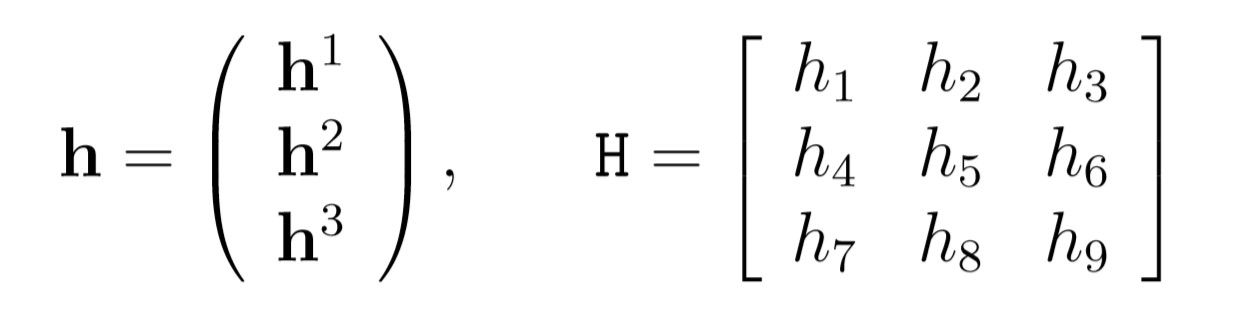
\includegraphics[width=0.49\textwidth]{FiguresIS/42.jpg}
    \caption{\cite{Richard2000} \todo{Beschreibung von h und H}}
\end{figure}

Um zweidimensionale Punkte mit dieser Matrix multiplizieren zu können müssen diese in die Homogene Darstellung gebracht werden. In dieser Darstellung ist der Punkt als Vektor mit einem inversen Streckungsfaktor w bestimmt. 
				$$[x1, x2, w]$$
Die $H$ Matrix muss nun aus den Punktkorrespondenzen bestimmt werden. Damit Sie vollständig bestimmt ist müssen mindestens vier Punktkorrespondenzen vorhanden sein.
Das Kreuzprodukt aus zwei gleichen Vektoren ist Null. Diese Eigenschaft macht man sich zu Nutze, um eine Lineare Lösung für die $H$-Matrix zu finden. Man kann also schreiben:
			$$ x‘ \times H x=0$$
Jede j-e Zeile der Matrix kann als $h_j^T$ bezeichnet werden dann kann man das Kreuzprodukt ausschreiben als:

\begin{figure}[ht]
    \centering
    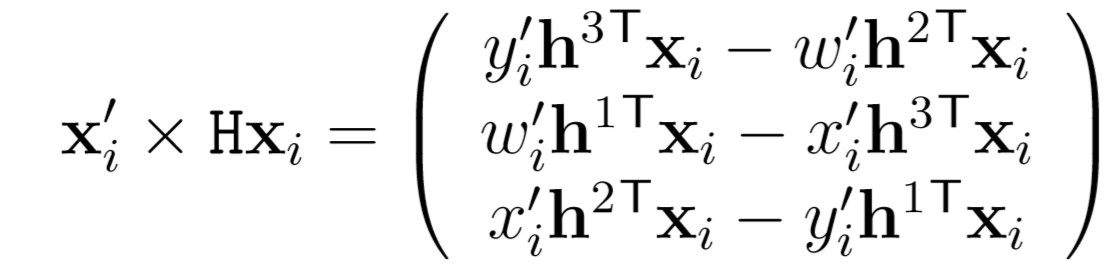
\includegraphics[width=0.49\textwidth]{FiguresIS/40.jpg}
    \caption{\cite{Richard2000}}
\end{figure}

Da $h_j^T\times x=x^T\times h_j$ ergibt das drei Gleichungen.  Man kann sie in Matrizenform schreiben als:
 
\begin{figure}[ht]
    \centering
    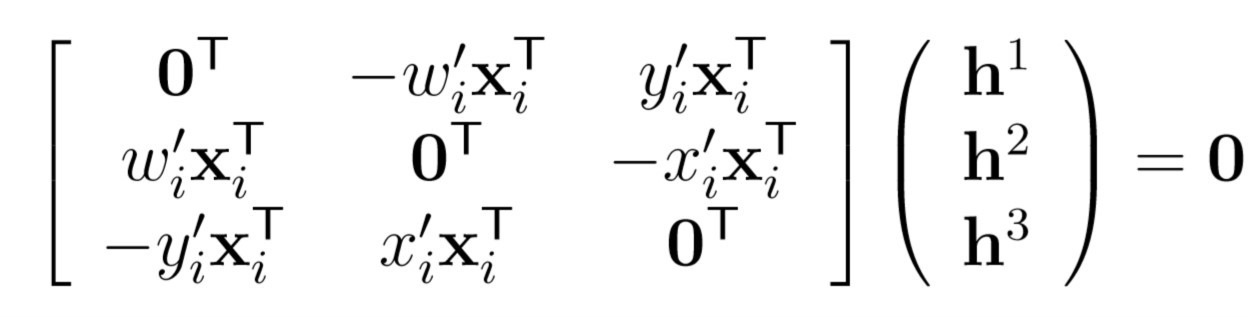
\includegraphics[width=0.49\textwidth]{FiguresIS/41.jpg}
    \caption{\cite{Richard2000}}
\end{figure}


Von den drei Gleichungen sind nur zwei linear unabhängig. Die dritte Zeile ergibt sich aus einer Linearkombination von den beiden anderen. Dann werden die Gleichungen zu:

\begin{figure}[ht]
    \centering
    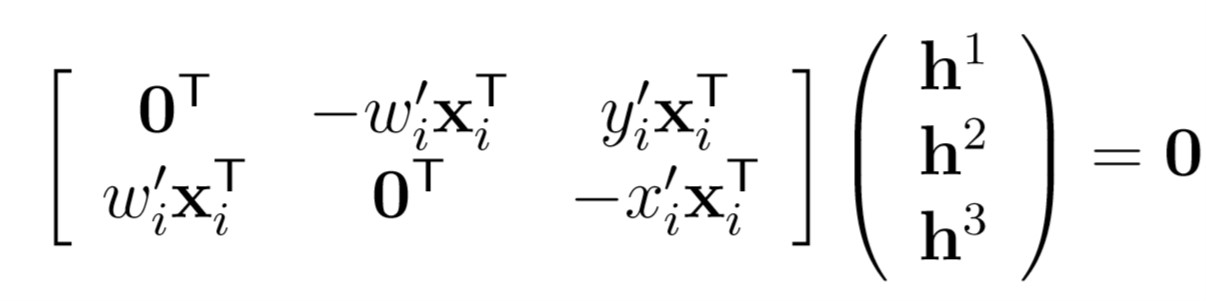
\includegraphics[width=0.49\textwidth]{FiguresIS/43.jpg}
    \caption{\cite{Richard2000}}
\end{figure}

Diese Gleichungen gelten für alle Punktkorrespondenzen in homogener Darstellung. Wählt man den inversen Streckungsfaktor w als 1 dann vereinfacht sich die Gleichung und die Punkte können als:
			$$[x, y, 1]$$
Dargestellt werden. Wobei $x$ und $y$ die Koordinaten aus dem Bild sind.

\subsection{Inhomogene Lösung}
Bis jetzt besteht das Gleichungssystem aus acht linear unabhängigen Gleichungen und neun unbekannten $h_j$. Für die inhomogene Lösung wird ein Eintrag von $h$ zu $h_j$=1 gesetzt. Das ist zulässig da die $H$-Matrix bis auf einen Skalierungsfaktor bestimmt ist und dieser beliebig gewählt werden kann. In unserer Implementierung wurde $h_9=1$ gesetzt. Somit bleibt ein Gleichungssystem mit acht Gleichungen und acht unbekannten übrig.
Dieses Gleichungssystem wird mithilfe einer Singulärwertzerlegung gelöst. Dazu wir die gesamte Matrix, die sich aus den Gleichungen ergibt in die Matrizen $U$, $D$ und $V$ zerlegt. Wobei $U$ und $V$ orthogonale Matrizen sind und $D$ eine Diagonalmatrix bestehend aus den Singulärwerten. Die Zerlegung wird so gemacht, dass die Einträge der Diagonalmatrix vom größten zum kleinsten sortiert sind. Die Lösung ist der Singulärvektor mit dem kleinsten Singulärwert. Das entspricht wegen der Sortierung der letzten spalte der Matrix $V$. Somit ist $h$ gelöst und muss nur noch wieder in $H$ umgewandelt werden indem die Einträge $h_1$, $h_2$ und $h_3$ gestapelt werden zu $H$.

\subsection{RANSAC Verfahren}
Bei der Suche von markanten Punkten in den Bildern und beim feature matching entstehen in einer Anwendung mit Fotos oft viele Fehler. Einerseits können die markanten Punkte z.B. aufgrund von Unschärfe eine ungenaue Position haben und andererseits können die Korrespondenzen falsch sein. Das passiert vor allem wenn das Bild sich wiederholende Strukturen (z.B. Gehwegplatten) hat. Dann kann es sein, dass Features verwechselt werden. Zusätzlich zu diesen beiden Fehlern spielt die Verzeichnung aufgrund der Krümmung der Kameralinse ebenfalls eine Rolle. Dadurch kann passieren, dass eine $H$-Matrix, die aus 4 matches in einem Teil des Bildes berechnet wurde zwar für diesen Teil gut gilt, allerdings passt dann der Rest der beiden Bilder nicht korrekt zusammen.
Um diesen Fehlern entgegenzuwirken wird mithilfe des RANSAC Algorithmus die $H$-Matrix gefunden, die möglichst fehlerfrei ist. RANSAC steht für RANdom SAmple Consensus. Der Algorithmus wird als robuste Schätzung bezeichnet, da er trotz einer großen Anzahl an fehlerhaften Samples ein gutes Ergebnis erreichen kann. Für die Schätzung der $H$ Matrix aus den matches von zwei Bildern sieht der Algorithmus wie folgt aus:

\textit{
Für n Wiederholungen:
\begin{itemize}
\item Es werden vier zufällige matches aus dem Set ausgewählt
\item Aus diesen wird eine $H$-Matrix berechnet.
\item Für jeden anderen match wird die geometrische Distanz berechnet. Jeder match dessen geometrische Distanz kleiner als der Mindestwert ist gilt als inlier.
\end{itemize}
Für beliebige Widerholungen:
\begin{itemize}
\item Die $H$-Matrix mit den meisten inliern wird ausgewählt.
\item Die $H$-Matrix wird nochmal berechnet unter Verwendung aller inlier.
\end{itemize}
}

Somit wird eine $H$-Matrix ausgewählt, die für möglichst viele der matches gilt. Der Algorithmus ist so robust, dass sogar bei fehlerraten von über 50\% gute Ergebnisse erreicht werden können. Das setzt voraus, dass keine systematischen Fehler auftreten, wie beispielweise eine fälschliche Verschiebung vieler matches um einen bestimmten Wert oder eine Rotation vieler matches. In diesem Fall wird der Algorithmus die $H$-Matrix falsch optimieren. Diese Fehler können nur sehr selten auftreten, wenn das Bild sich sehr wiederholende und ähnliche Strukturen aufweist. Man kann solche Fehler sehr leicht am Ergebnisbild erkennen. Abhilfe kann hier dann nur ein komplexerer feature matching Algorithmus schaffen, der die Strukturen besser unterscheiden kann.

\subsubsection{Parameter im RANSAC Verfahren}
Im RANSAC Verfahren werden für zufällige Punktekombinationen $H$-Matrizen berechnet. Der Zufall ist deswegen wichtig, da die Anzahl der Kombinationen mit der vierten Potenz der Anzahl von matches steigt. Eine testweise Implementierung eines “Brute Force Sample Consensus” der alle möglichen $H$-Matrizen berechnet und die beste auswählt, dauert bereits bei einer kleinen Anzahl von 17 matches etwa fünf Minuten auf meinem Rechner. Durch zufällige Auswahl der Punkte soll sichergestellt werden, dass mit der  Wahrscheinlichkeit $p$ eine $H$-Matrix berechnet wird, die ein inlier ist, also hinreichend genau ist. Um das sicherstellen zu können muss eine Mindestanzahl an 4-Punkt-Kombinationen geprüft werden. Nimmt man an dass $s$ die Anzahl der Punkte ist, die für die Berechnung einer $H$-Matrix benötigt werden und $\eta$ die geschätzte Menge an Ausreißern dann lässt sich die Mindestanzahl über die folgende Formel berechnen:
$$N=log(1-p)/log(1-(1-\eta)^s)$$
Ein weiterer Parameter, der für den RANSAC festgelegt werden muss ist die Schwelle für die geometrische Distanz, ab der ein Punkt als inlier gilt. Diese Schwelle sollte theoretisch $5.99*\sigma ^2$ betragen, da aber Sigma am Anfang der Berechnung nicht gegeben ist wurde die Schwelle durch probieren auf 4 festgelegt.

\subsubsection{Geometrische Distanz}
Um messbar zu bestimmen wie gut eine $H$-Matrix sich für eine Bildtransformation eignet, kann man die matches verwenden. Jedes Punktepaar einer Korrespondenz, besteht aus dem Punkt $x$ auf dem ersten Bild und dessen Entsprechung $y$ auf dem zweiten Bild. Die $H$-Matrix beschreibt die Transformation von $x$ nach $y$. Wären die matches und die Matrix fehlerfrei dann würde exakt gelten:
$$x H= y$$
Aufgrund von Ungenauigkeiten und Fehlern wird $x$ durch die Transformation mit $H$ abgebildet auf einen Punkt $x‘$, der von $y$ um den Abstand $d$ entfernt ist. Beim geometrischen Abstand wird einmal $x$ zu $x‘$ transformiert und einmal $y$ zu $ y‘$ rücktransformiert und es wird der Abstand zwischen den sich ergebenden Punkten und den tatsächlichen gebildet. Dieser Abstand wird dann quadratisch addiert. So ergibt sich der geometrische Abstand. Dies Summe über alle Punkte entspricht dann dem geometrischen Fehler. 

\begin{figure}[ht]
    \centering
    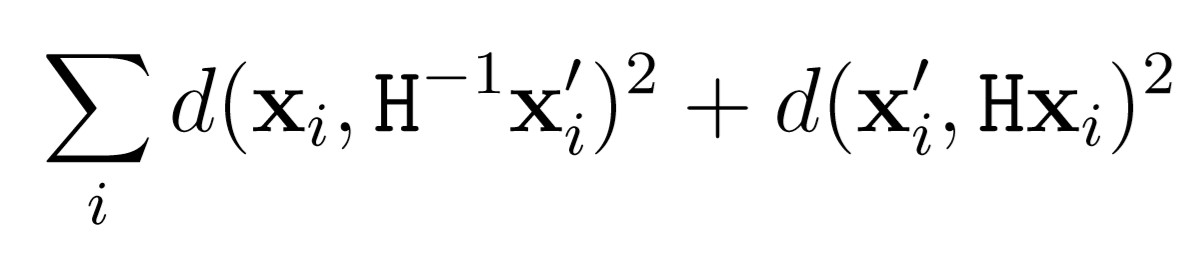
\includegraphics[width=0.49\textwidth]{FiguresIS/47.jpg}
    \caption{\cite{Richard2000}}
\end{figure}

Über diesen kann dann bestimmt werden ob ein Punkt für eine $H$-Matrix ein inlier ist oder nicht. Berechnet man den Erwartungswert und die Standartabweichung der geometrischen Distanz für alle Bildkorrespondenzen für eine $H$-Matrix so erhält man ein Maß für die Güte dieser $H$-Matrix.

\subsection{Bildtransformation}
Sobald die $H$-Matrix fertig ist müssen die Bilder überlagert werden. Dazu muss das zweite Bild mit der $H$-Matrix transformiert werden. Beim Transformieren eines ganzen Bildes muss jeder Pixel an seine neue Position gebracht werden. Dabei kann es auftreten, dass es im neuen Bild ungefüllte Positionen, also Lücken gibt. Um dem entgegenzuwirken wird bilineare Interpolation verwendet, sodass keine Lücken entstehen. Ein weiteres Problem, das entstehen kann ist, dass das transformierte Bild sich im negativen Bereich befindet. Das ist von der Datenstruktur unmöglich abzuspeichern. Das folgende Vorgehen ist so gemacht, dass beide oben beschriebene Probleme nicht auftreten.
Zuerst wird das fertige gemeinsame Bild als Matrix von Nullen festgelegt. Dazu werden die Eckpunkte des zweiten Bildes transformiert. Aus Den Eckpunkten des ersten Bildes und denen des transformierten zweiten Bildes lässt sich die resultierende Bildgröße berechnen. Sind die Punkte des transformierten zweiten Bildes negativ in einer oder beiden Dimensionen, so ist das der Offset, der auf beide Bilder addiert wird und diese in positive Richtung verschiebt.
Nun werden beide Bilder auf den canvas übertragen. Das Vorgehen ist so:
Für alle Pixel $p`$ innerhalb des transformierten Bildbereichs auf dem canvas:
Transformiere $p`$ zurück zu $p$ mit der inversen von H
Wenn $p$ innerhalb des nicht transformierten Bildes liegt
	Führe bilineare Interpolation zwischen den umliegenden Pixeln von $p$ aus
	Schreibe das Ergebnis in $p`$

Auf diese Weise können wird das resultierende Gesamtbild aus dem negativen Bereich geschoben und es können niemals Lücken zwischen den Pixeln entstehen. Es muss jedoch darauf hingewiesen werden, dass diese Art von Bildtransformation deutlich langsamer ist als entsprechende Bibliotheksfunktionen, da solche Operationen wie Transformation und bilineare Interpolation normalerweise durch die Grafik-Pipeline erledigt werden, welche das hardwarebeschleunigt ausführt.

\clearpage

